\documentclass[11pt,a4paper]{article}
\usepackage{fontspec}
\setmainfont{Times New Roman}
\setmonofont{Courier New}[Scale=0.88]
\usepackage[spanish]{babel}
\usepackage[margin=1.9cm]{geometry}
\usepackage{xcolor}
\usepackage{longtable,array,booktabs}
\usepackage{enumitem}
\usepackage{fancyhdr}
\usepackage{titlesec}
\usepackage{graphicx}
\usepackage{pdflscape}
\usepackage{needspace}
\usepackage{url}
\urlstyle{tt}

\graphicspath{{../}}
\definecolor{azul}{RGB}{31,73,125}
\definecolor{amar}{RGB}{255,248,220}
\definecolor{rojo}{RGB}{160,30,30}
\definecolor{verde}{RGB}{30,110,50}
\definecolor{naranja}{RGB}{190,110,0}

\titleformat{\section}{\Large\bfseries\color{azul}}{\thesection.}{0.5em}{}[\vspace{-0.3em}\color{azul}\titlerule]
\titleformat{\subsection}{\large\bfseries\color{azul}}{\thesubsection}{0.5em}{}
\setlength{\parindent}{0pt}
\setlength{\parskip}{4pt}
\setlength{\tabcolsep}{3pt}
\emergencystretch=4em
\setlist{itemsep=1pt,topsep=2pt}
\pagestyle{fancy}
\fancyhf{}
\fancyhead[L]{\small RAC -- Diseño de una red corporativa: memoria técnica}
\fancyhead[R]{\small Versión 4 (8-nov-2026)}
\fancyfoot[C]{\small\thepage}

\newcommand{\cod}[1]{\texttt{#1}}
\newcommand{\ok}{\textcolor{verde}{\textbf{Aplicado y probado}}}
\newcommand{\dis}{\textcolor{azul}{\textbf{Diseñado}}}
\newcommand{\pen}{\textcolor{rojo}{\textbf{Pendiente}}}
\newcommand{\sinp}{\textcolor{naranja}{\textbf{Sin probar}}}
\newcommand{\hecho}{\textcolor{verde}{\textbf{Resuelto}}}
\newcommand{\abierto}{\textcolor{rojo}{\textbf{Abierto}}}
\newsavebox{\notebox}
\newenvironment{nota}{\par\medskip\noindent\begin{lrbox}{\notebox}\begin{minipage}{0.95\textwidth}\small}{\end{minipage}\end{lrbox}\fcolorbox{black!30}{amar}{\usebox{\notebox}}\par\medskip}

\begin{document}

\begin{center}
{\Huge\bfseries Diseño de una red corporativa}\\[2pt]
{\Large Memoria técnica: diseño, estado de implementación y pasos pendientes}\\[2pt]
{\large Redes de Acceso y Corporativas \quad|\quad Proyecto en GNS3 \quad|\quad versión 4, 8 de noviembre de 2026}\\[2pt]
{\normalsize Equipo: Javi, Pepe y Manu}
\end{center}

\begin{nota}
\textbf{Cómo leer este informe.} Cada elemento está en uno de cuatro estados:
\dis\ (decidido en el diseño, aún no configurado),
\sinp\ (configurado o con scripts generados, sin comprobar en los routers),
\ok\ (configurado en los routers de GNS3 \textbf{y} comprobado con pruebas, con resultado guardado) y
\pen\ (no empezado).
A 8 de noviembre de 2026 \textbf{solo está «aplicado y probado» la fase 1}: direcciones, enlaces, WAN con dos proveedores y salida a Internet (49 de 49 pruebas de ping correctas). El resto es diseño o plan. Nada de lo que aquí se dice de disponibilidad está aún medido.
\end{nota}

\section{Resumen ejecutivo}
Proponemos una red corporativa para una empresa con una \textbf{sede principal} (HQ, 200 puestos) y dos \textbf{sucursales} (B1, 50 puestos; B2, 10 puestos), con acceso a Internet, web pública, servicios de almacenamiento y cómputo, y acceso seguro para teletrabajadores. La red es jerárquica y modular (borde, firewall, core, distribución, acceso) y está \textbf{duplicada de extremo a extremo}: dos proveedores de Internet (ISP1 e ISP2), y en cada sede dos routers de salida, dos pasarelas y dos caminos hasta cada switch de acceso. El objetivo que nos hemos puesto es una \textbf{disponibilidad de 0,999} (unas 8,8 horas de caída al año). Es un objetivo propio: el enunciado solo pide «disponibilidad» sin cifra.

La simulación se hace en GNS3 (no en Packet Tracer, que limitaría la nota al 85\,\%): \textbf{51 dispositivos y 71 enlaces}, con 14 routers MikroTik CHR, switches de acceso Open vSwitch y servicios en contenedores. La configuración se aplica \textbf{con scripts} y se comprueba también con scripts, de modo que la red es reproducible.

\textbf{Dónde estamos.} La topología está montada y la fase 1 está aplicada y probada. Quedan por hacer, por este orden: encaminamiento OSPF, VLAN con RSTP y pasarelas redundantes, salida a Internet con firewall, túneles y teletrabajo, observabilidad y autenticación, y las pruebas de fallo que demuestren la disponibilidad (secciones~\ref{sec:estado} y~\ref{sec:pasos}).

\section{Objetivo principal y alcance}
\textbf{Objetivo.} Diseñar e implementar desde cero una red corporativa segura, escalable, disponible y gestionable que dé servicio a tres sedes, a invitados y a teletrabajadores, con servicios propios (almacenamiento, cómputo y web pública) y con monitorización y detección de eventos de seguridad en toda la red.

\textbf{Alcance.} LAN de cada sede, WAN entre sedes, DMZ y acceso desde Internet, para toda la empresa. Queda fuera el despliegue físico real: se trabaja en simulación.

\section{Estado de avance}\label{sec:estado}
\begingroup\footnotesize
\begin{longtable}{@{}p{0.9cm}p{6.6cm}p{2.9cm}p{6.1cm}@{}}
\toprule
\textbf{Fase} & \textbf{Contenido} & \textbf{Estado} & \textbf{Evidencia}\\
\midrule
\endhead
0 & Topología en GNS3 (51 nodos, 71 enlaces); plan de direcciones; repositorio y scripts de aplicación y prueba & \ok\ (topología) & Proyecto \cod{RAC\_Red\_HA}; abre y arranca\\
1 & Direcciones de los enlaces, loopbacks, WAN con dos ISP, rutas por defecto provisionales & \ok & 49 de 49 pruebas de ping (apéndice~\ref{ap:pruebas}); log de cada ejecución\\
2 & OSPFv2 y OSPFv3 en HQ; BFD & \sinp\ (scripts generados) & --\\
3 & Nivel 2 y pasarelas: RSTP, VLAN, VRRP, DHCP y SLAAC & \pen & --\\
4 & Salida a Internet (NAT), firewall, DMZ, política entre zonas & \pen & --\\
5 & Túneles WireGuard a B1 y B2; teletrabajo; OSPF en sucursales & \pen & --\\
6 & Observabilidad (Prometheus, Grafana) y autenticación (FreeRADIUS) & \pen\ (nodos creados, sin configurar) & --\\
7 & Pruebas de fallo, medición y cálculo de disponibilidad & \pen & --\\
8 & Memoria final (plantilla de Prado), presupuesto, presentación & \pen & --\\
\bottomrule
\end{longtable}
\endgroup

\subsection{Qué está aplicado y cómo se comprobó (fase 1)}
\textbf{Método.} Los ficheros de configuración (\cod{.rsc}, uno por router y fase) se envían a cada router con un script (\cod{push\_config.py}) que se conecta a su consola, entra con el usuario \cod{admin} y ejecuta los comandos, anotando cada resultado en un registro. Otro script (\cod{test\_fase1.py}) lanza \cod{/ping <destino> count=3} desde cada router y da la prueba por buena si responden los tres paquetes. Las pruebas salen del mismo plan de direcciones que generó la configuración.

\textbf{Resultado} (ejecución del 8 de noviembre de 2026):
\begingroup\small
\begin{longtable}{@{}p{5cm}p{3cm}p{3cm}@{}}
\toprule
\textbf{Grupo de pruebas} & \textbf{Pruebas} & \textbf{OK}\\
\midrule
\endhead
enlaces HQ & 32 & 32\\
WAN & 12 & 12\\
sedes & 3 & 3\\
Internet & 2 & 2\\
\textbf{Total} & \textbf{49} & \textbf{49}\\
\bottomrule
\end{longtable}
\endgroup

Los RTT medios entre routers vecinos están entre 0,6 y 1,6\,ms. Desde ISP1 e ISP2 a 8.8.8.8 salieron 17,3 y 19,7\,ms: ISP1 sale por el NAT de GNS3 e ISP2 lo hace a través de ISP1. En el apéndice~\ref{ap:pruebas} está la tabla completa de las 49 pruebas.

\textbf{Qué prueba y qué no.} Estas pruebas demuestran que las direcciones están bien puestas y que cada cable de GNS3 coincide con el puerto previsto del plan. \textbf{No} demuestran todavía encaminamiento, redundancia ni seguridad: son sólo conectividad entre vecinos.

\section{Trazabilidad con el enunciado}
\begingroup\footnotesize
\begin{longtable}{@{}p{3.3cm}p{8.4cm}p{4.8cm}@{}}
\toprule
\textbf{Requisito del enunciado} & \textbf{Cómo lo cubrimos} & \textbf{Estado}\\
\midrule
\endhead
Sede principal y dos sedes remotas B1 y B2 & Tres sedes unidas por túneles sobre dos ISP simulados & Topología \ok; túneles \pen\\
200, 50 y 10 puestos fijos & Reparto por departamento y VLAN; \textbf{B1 y B2: reparto supuesto, por confirmar} & \dis; en GNS3 un equipo representante por departamento\\
Conexiones adicionales para internos e invitados & VLAN de invitados y un punto de acceso Wi-Fi por sede; invitados sólo con Internet, sin acceso interno & \dis; AP simulado\\
5 departamentos en HQ y B1; sólo investigación y cursos en B2 & VLAN 10 a 50 en HQ y B1; VLAN 10 y 40 en B2 & \dis\\
Servidores de almacenamiento y cómputo con alta disponibilidad; cómputo sólo para investigación y soporte & Pareja de servidores por servicio, cada uno en un switch distinto y con doble enlace; regla del firewall que limita el cómputo a las VLAN 10 y 50 & Topología \ok; regla \pen\\
Direccionamiento dinámico y estático & DHCP en las pasarelas (pool .100--.250), direcciones fijas para servidores y equipos de red, SLAAC en IPv6 & Enlaces y loopbacks \ok; DHCP \pen\\
Encaminamiento intra e inter-sedes & OSPF (v2 y v3) en cada sede y entre sedes por los túneles & \sinp\\
B2 sólo IPv4; HQ y B1 con IPv6 & HQ y B1 en doble pila; B2 sin IPv6 & Aplicado en los enlaces \ok\\
Web de la empresa expuesta públicamente & Servidor web en la DMZ, publicado con NAT estático y filtrado & Nodo creado; configuración \pen\\
Internet para empleados e invitados & NAT/PAT en los bordes (en IPv6, sin NAT) & Salida de los ISP \ok; NAT en bordes \pen\\
Teletrabajadores desde Internet & VPN WireGuard hasta HQ & \dis; WireGuard \textbf{por verificar} en la documentación oficial\\
Pico de 500\,kbps por puesto & Dimensionado de enlaces (sección~\ref{sec:dim}) & Cálculo \dis; prueba de tráfico \pen\\
Todas las comunicaciones seguras & Túneles cifrados, SSH con autenticación, SNMPv3, TLS en la web & \dis\\
Monitorización, securización y detección de eventos & Prometheus y Grafana, firewall con registro, RADIUS; IDS/IPS por decidir & \dis; nodos creados\\
Escalabilidad, disponibilidad, seguridad, gestionabilidad & Matriz de la sección~\ref{sec:nofun} & Parcial\\
Memoria con las secciones del enunciado y decisiones justificadas & Este documento, que sigue su estructura; presupuesto sin precios & Parcial\\
Presentación oral de las problemáticas & Sección~\ref{sec:probl} & Material \dis; presentación \pen\\
Proyecto en el simulador elegido & \cod{RAC\_Red\_HA.gns3} + scripts en el repositorio & \ok\\
Plantilla \LaTeX\ de Prado y participación de cada miembro & No tenemos aún la plantilla; reparto propuesto en la sección~\ref{sec:plan} & \pen\\
\bottomrule
\end{longtable}
\endgroup

\section{Requisitos de diseño}
\subsection{Requisitos de negocio y técnicos}
\begin{itemize}
\item \textbf{Negocio:} servicio fiable a 260 puestos fijos y a invitados, web pública, teletrabajo y reducción del coste operativo mediante gestión automatizada.
\item \textbf{Técnicos:} escalabilidad, disponibilidad, seguridad y gestionabilidad (sección~\ref{sec:nofun}), con la disponibilidad como requisito que condiciona la topología (sección~\ref{sec:disp}).
\item \textbf{Comunidades de usuarios:} cinco departamentos, invitados y teletrabajadores. \textbf{Aplicaciones:} web pública, almacenamiento, cómputo, monitorización y autenticación.
\end{itemize}

\subsection{Dimensionado del tráfico}\label{sec:dim}
Con el pico de 500\,kbps por puesto fijo y sumando el \textbf{caso peor} (todos a la vez):
\begin{longtable}{@{}p{5cm}p{3.2cm}p{3.7cm}p{4.5cm}@{}}
\toprule
\textbf{Tramo} & \textbf{Puestos} & \textbf{Pico agregado} & \textbf{Enlace propuesto}\\
\midrule
\endhead
HQ completa & 200 & 100\,Mbps & Enlaces internos de 1\,Gbps\\
Acceso HQ 1 (VLAN 10, 20 y 30) & 60 + 35 + 35 $=$ 130 & 65\,Mbps & 1\,Gbps ($\approx$6,5\,\%)\\
Acceso HQ 2 (VLAN 40 y 50) & 30 + 40 $=$ 70 & 35\,Mbps & 1\,Gbps ($\approx$3,5\,\%)\\
B1 & 50 & 25\,Mbps & 1\,Gbps interno; túnel hacia HQ\\
B2 & 10 & 5\,Mbps & 100\,Mbps o más; túnel hacia HQ\\
Salida de HQ a Internet y túneles & 100 + 25 + 5 & hasta 130\,Mbps & $\geq$200\,Mbps por router de borde (margen del 50\,\%)\\
\bottomrule
\end{longtable}
Los invitados y teletrabajadores no cuentan aquí: el enunciado fija el pico sólo para los puestos fijos. Las velocidades son una \textbf{propuesta}. En el simulador los enlaces no están limitados, y además la licencia gratuita del CHR limita cada interfaz a 1\,Mbps de subida, así que \textbf{el rendimiento a estas velocidades no se puede medir sin licencia} (sección~\ref{sec:lic}).

\section{Arquitectura lógica}
\begin{landscape}
\begin{center}
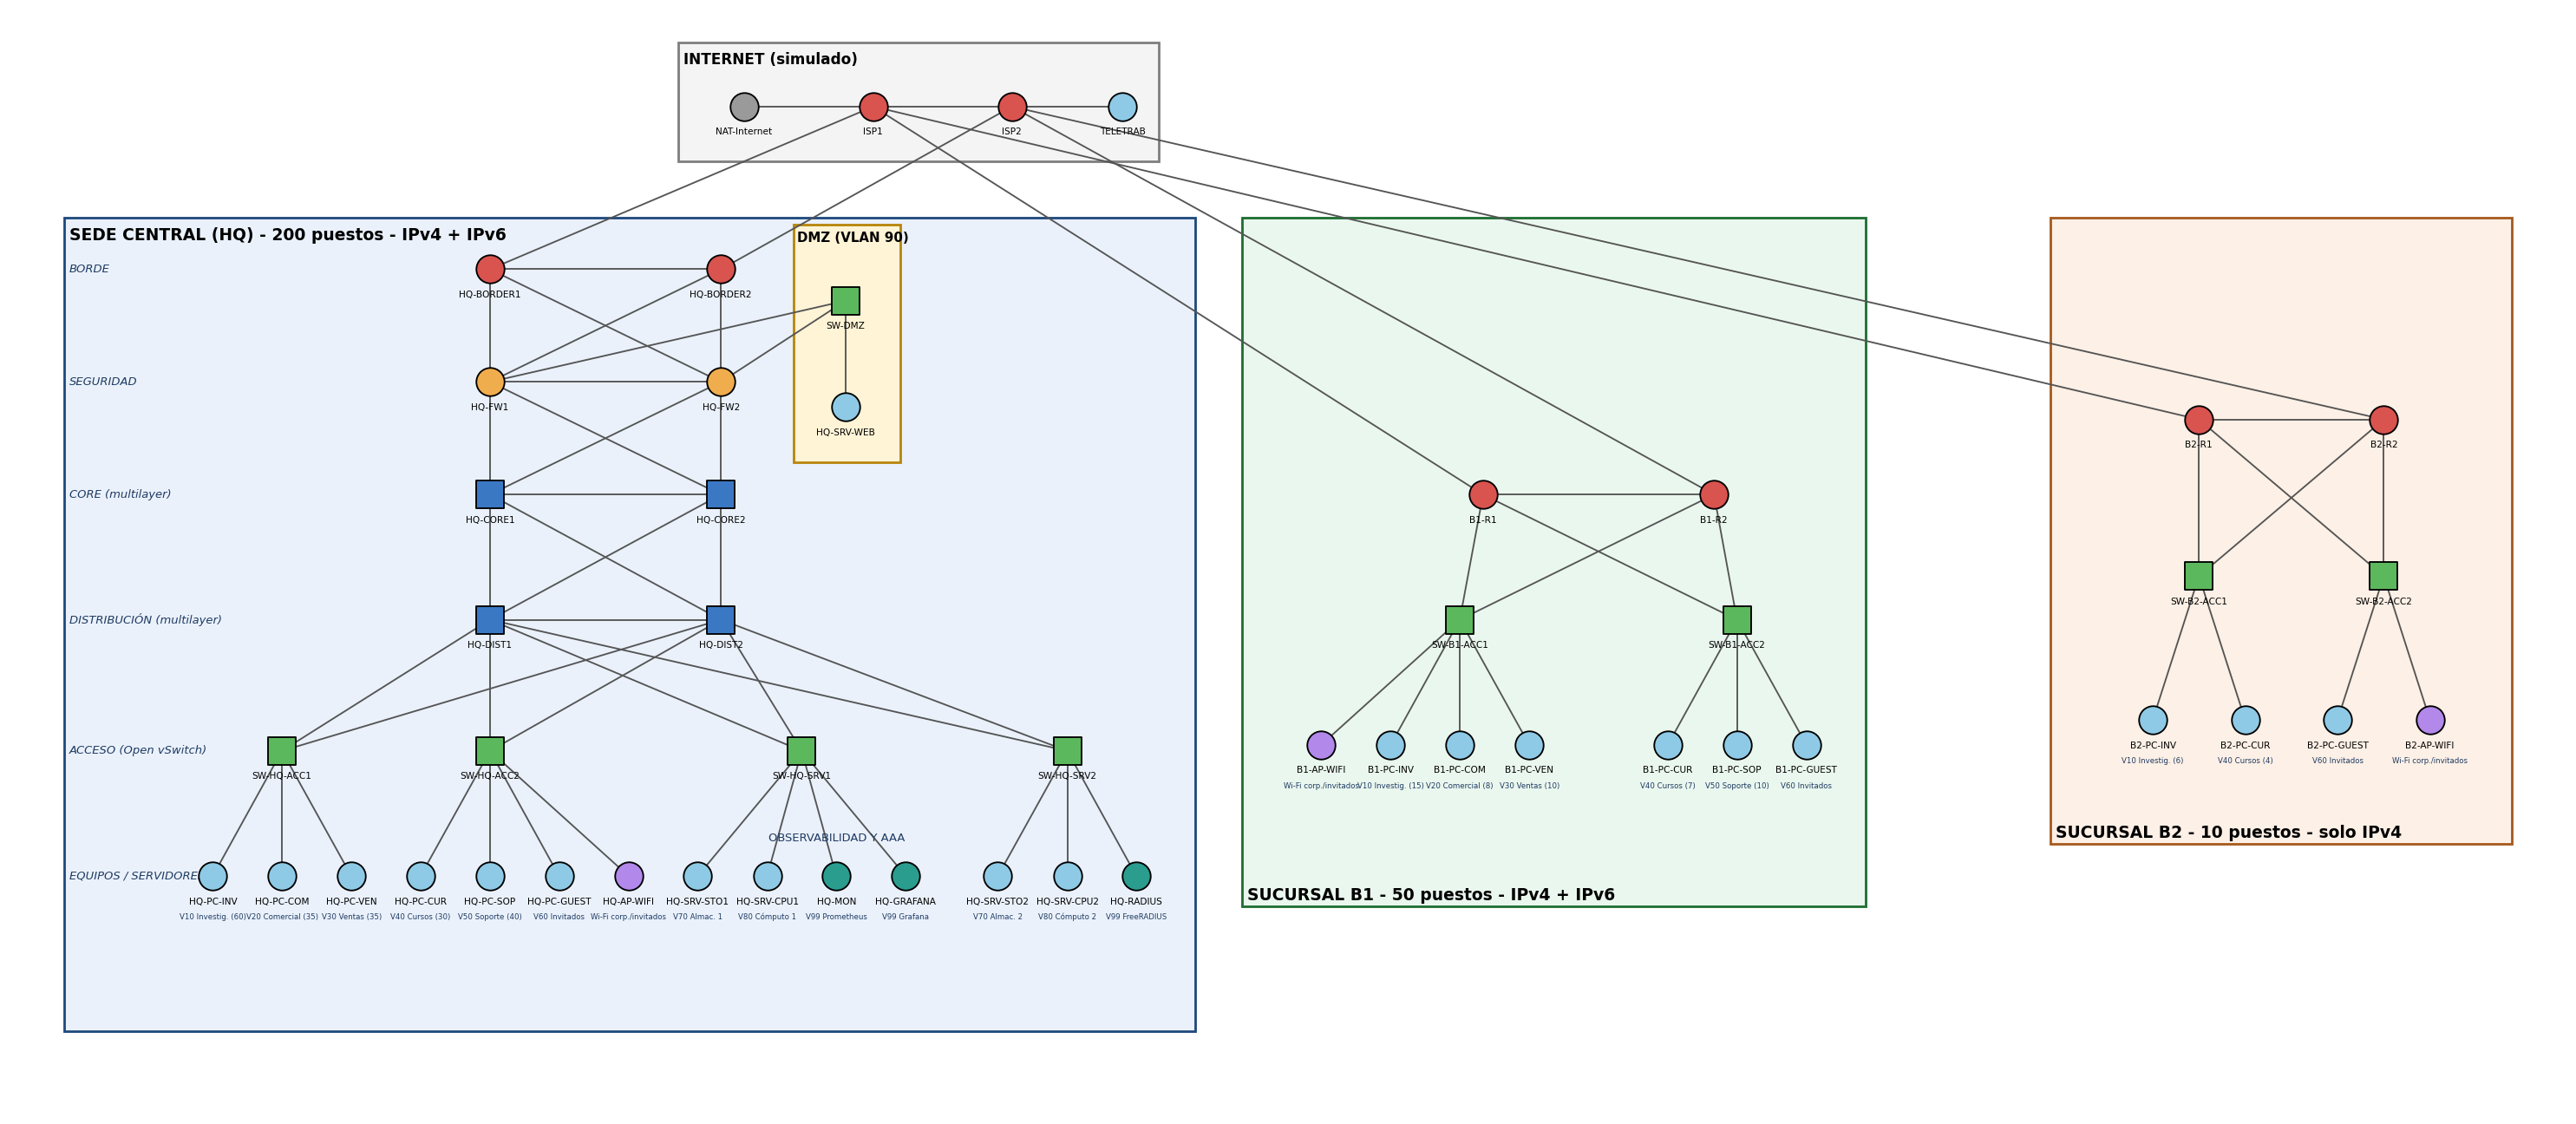
\includegraphics[width=24.5cm]{topologia_HA.png}
\end{center}
\vspace{-0.5em}
{\small Rojo: routers. Naranja: firewalls (CHR). Azul (cuadrado): switches multicapa. Verde (cuadrado): Open vSwitch. Celeste: equipos y servidores. Turquesa: servicios (Prometheus, Grafana, FreeRADIUS). Morado: puntos de acceso Wi-Fi (simulados). Todos los enlaces redundantes están activos.}
\end{landscape}

La red es jerárquica: \textbf{borde} (routers que dan salida a Internet y terminan los túneles), \textbf{seguridad} (firewalls), \textbf{core}, \textbf{distribución} y \textbf{acceso}. Entre capas los enlaces son enrutados, y el nivel 2 sólo llega hasta el switch de acceso. Cada nivel está duplicado:
\begin{itemize}
\item \textbf{Internet:} ISP1 e ISP2, interconectados. HQ-BORDER1, B1-R1 y B2-R1 salen por ISP1; HQ-BORDER2, B1-R2, B2-R2 y el teletrabajador por ISP2. ISP1 da la salida real a Internet (NAT de GNS3).
\item \textbf{HQ:} 2 bordes, 2 firewalls conectados a los dos bordes y a los dos core (malla completa), 2 core, 2 distribución, 3 switches de acceso y 2 de servidores, cada uno con un enlace a DIST1 y otro a DIST2.
\item \textbf{B1 y B2:} 2 routers cada una (cada router hace de borde y de pasarela, con su propio ISP) y 2 switches de acceso conectados a los dos routers.
\item \textbf{Servidores:} almacenamiento 1 y cómputo 1 en SRV1; almacenamiento 2 y cómputo 2 en SRV2. Así un fallo de un switch no deja sin servicio a ninguno de los dos.
\end{itemize}

\subsection{Decisiones y alternativas}\label{sec:decis}
\begingroup\footnotesize
\begin{longtable}{@{}p{2.5cm}p{3.3cm}p{4.2cm}p{6.5cm}@{}}
\toprule
\textbf{Decisión} & \textbf{Elegido} & \textbf{Alternativas} & \textbf{Por qué}\\
\midrule
\endhead
Routers y switches multicapa & MikroTik CHR 7.22.1 & Cumulus VX, FRR sobre Linux, Cisco IOSvL2 o Catalyst 9000v, Arista vEOS/cEOS & Ya está en el catálogo de GNS3 y es ligero (256\,MB). Los de Cisco necesitan imagen con cuenta y licencia. Soporta lo que necesitamos (routing, VRRP, OSPF, BFD, WireGuard); en la práctica sólo hemos probado direccionamiento y conectividad hasta ahora\\
Switches de acceso & Open vSwitch & Switch integrado de GNS3, CHR en modo bridge & Soporta VLAN y STP, apenas consume y se usó en clase. El integrado no tiene STP. \textbf{Que el OVS del contenedor active RSTP está por comprobar}\\
Firewall perimetral & Pareja de CHR con VRRP (provisional) & OPNsense 26.1, pfSense, FortiGate & Abre sin importar imágenes y sin RAM extra. \textbf{No incluye IPS}: OPNsense lo haría (Suricata, según su manual) pero necesita una imagen de unos 3\,GB. Decisión abierta (sección~\ref{sec:preg})\\
Dos proveedores de Internet & ISP1 e ISP2 & Un solo ISP con dos enlaces & El ISP es si no un único punto de fallo para toda la empresa. Cuesta un router más en la simulación\\
Redundancia de pasarelas & VRRP por VLAN con reparto de carga & HSRP/MHSRP (usado el año pasado) & RouterOS implementa VRRP; HSRP es propietario de Cisco\\
Encaminamiento & OSPFv2 y OSPFv3 con BFD & RIP, BGP, rutas estáticas & OSPF converge bien en esta escala. BFD acelera la detección del fallo (las diapositivas de DDR piden convergencia rápida). \textbf{Sin probar}\\
VPN entre sedes y teletrabajo & WireGuard, dos túneles por sede (uno por ISP) & IPsec, OpenVPN & Configuración corta. \textbf{Sólo he encontrado fuentes de terceros} sobre su soporte en RouterOS~7: hay que verificarlo en la documentación oficial\\
Direccionamiento IPv6 & GUA + ULA & Sólo GUA, o sólo ULA con NAT66 & ULA para infraestructura y servicios internos (estable aunque cambie el ISP), GUA para Internet. Riesgo en la sección~\ref{sec:gua}\\
Observabilidad & Prometheus + Grafana & Zabbix, LibreNMS & Estándar actual para métricas y paneles; contenedores ya creados. \textbf{Cómo recoger las métricas de los routers (por ejemplo SNMP) no está decidido}\\
\bottomrule
\end{longtable}
\endgroup

\subsection{¿Bastan los MikroTik?}\label{sec:lic}
Para este trabajo, sí funcionalmente: routing, VRRP, OSPF, BFD y WireGuard son características de RouterOS. Matices:
\begin{itemize}
\item \textbf{Licencia del CHR.} La versión gratuita limita a \textbf{1\,Mbps de subida por interfaz}; las licencias P1 y P10 suben el límite a 1 y 10\,Gbps, y hay una prueba de 60 días (manual de MikroTik). Sirve para conectividad y para medir recuperación, \textbf{no} para medir rendimiento a 100\,Mbps. Decisión del equipo: probar sólo funcionalidad y razonar el rendimiento por cálculo.
\item \textbf{Un CHR no es un switch multicapa real:} el reenvío es por software. En el diseño físico habría que elegir hardware con conmutación en chip; los modelos no están elegidos.
\item \textbf{IPS:} RouterOS no sirve como IPS; por eso OPNsense sigue siendo una opción.
\end{itemize}

\section{Disponibilidad}\label{sec:disp}
\subsection{Objetivo y definición}
\textbf{Objetivo: 0,999} (8,76 horas de caída al año, unos 43 minutos al mes). No viene del enunciado. Lo medimos como \textbf{disponibilidad del servicio de red de cada sede}: la sede mantiene conectividad a sus servicios, a las otras sedes y a Internet, las 24 horas. Que un puerto concreto se quede sin servicio no cuenta como caída de la sede, pero sí lo contamos por separado como disponibilidad de un puesto.

\subsection{Modelo}
Siguiendo el Tema~2 de DDR: en serie, la disponibilidad es el producto $A=\prod A_i$; en paralelo, $A=1-\prod(1-A_i)$. De ahí dos consecuencias: una cadena en serie nunca supera a su elemento más débil, y sólo compensa replicar el elemento que limita.

\textbf{Ejemplo ilustrativo para B1.} \textbf{Los valores son supuestos míos, no medidos ni de un fabricante:} enlace WAN 0,995; router o switch 0,999. Un puesto de B1 depende de WAN, router de salida, router de pasarela y switch de acceso:
\begin{center}
\begin{tabular}{@{}p{7.7cm}p{3.1cm}p{3.5cm}@{}}
\toprule
\textbf{Situación} & \textbf{Disponibilidad} & \textbf{Caída al año}\\
\midrule
Diseño anterior (un solo camino por sede) & 0,9920 & $\approx$ 70 horas\\
Diseño actual, puesto detrás de \textbf{un} switch de acceso & 0,99897 & $\approx$ 9,0 horas\\
Diseño actual, \textbf{sede} (basta un switch de acceso vivo) & 0,99997 & $\approx$ 14 minutos\\
\bottomrule
\end{tabular}
\end{center}
Conclusiones del ejemplo: (1) con un solo camino no se llega a 0,999 aunque cada elemento valga 0,999; (2) con todo duplicado la \textbf{sede} supera 0,999 con margen; (3) un \textbf{puesto} queda justo por debajo (0,99897), porque su switch de acceso es un elemento en serie: para que el puesto llegue a 0,999 haría falta un switch de al menos 0,99903. Es el elemento más débil que queda, y la regla de DDR dice que es el siguiente a replicar o a mejorar.

\subsection{Límites del modelo}
La fórmula en paralelo supone fallos independientes, y no lo son: errores de configuración, fallos de software y causas comunes afectan a la vez a los dos elementos de una pareja. Según los resúmenes del trabajo de \textit{Gill, Jain y Nagappan} (SIGCOMM 2011, registros de fallos de decenas de centros de datos), la redundancia sólo reduce en torno a un 40\,\% el impacto mediano de un fallo (\textbf{cifra tomada de resúmenes; no he leído el artículo completo}); \textit{Turner et al.} (SIGCOMM 2010) estudian fallos en una red de más de 200 routers. Por eso este informe \textbf{no} da el 0,999 por demostrado con la fórmula: lo que se hará es medir tiempos de recuperación reales con pruebas de fallo (sección~\ref{sec:pruebas}) y comparar con el presupuesto de caída.

\section{Plan de direccionamiento}
Regla común: el tercer octeto IPv4 es el número de VLAN. Cada sede lleva un bloque propio para poder resumirlo.

\subsection{Prefijos}
\begin{longtable}{@{}p{2.2cm}p{4.4cm}p{9.9cm}@{}}
\toprule
\textbf{Sede} & \textbf{IPv4} & \textbf{IPv6}\\
\midrule
\endhead
HQ & \cod{10.1.0.0/16} & GUA \cod{2001:db8:1::/48}; ULA \cod{fdce:f6ae:a8d8:1000::/52}\\
B1 & \cod{10.2.0.0/16} & GUA \cod{2001:db8:2::/48}; ULA \cod{fdce:f6ae:a8d8:2000::/52}\\
B2 & \cod{10.3.0.0/16} & No (sólo IPv4)\\
Túneles y teletrabajo & \cod{10.255.0.0/16} & ULA \cod{fdce:f6ae:a8d8:ff00::/56}\\
Internet simulado & \cod{203.0.113.0/24} & \cod{2001:db8:ffff::/48}\\
\bottomrule
\end{longtable}
Las GUA (\cod{2001:db8::/32}) y las IPv4 «públicas» (\cod{203.0.113.0/24}) son rangos de documentación, válidos para simular. La ULA es un identificador aleatorio generado para esta empresa (RFC~4193).

\subsection{Infraestructura aplicada (fase 1)}\label{sec:infra}
\textbf{Estado: \ok.} Loopbacks y enlaces entre routers usan \textbf{ULA} en IPv6 (decisión del equipo) y /30 en IPv4. En los enlaces, cada extremo toma una dirección de un /127 (RFC~6164). Estas tablas se extraen \textbf{de los ficheros de configuración aplicados}.

\textbf{Loopbacks}
\begingroup\footnotesize
\begin{longtable}{@{}p{3.4cm}p{4cm}p{6cm}@{}}
\toprule
\textbf{Router} & \textbf{Loopback IPv4} & \textbf{Loopback IPv6 (ULA)}\\
\midrule
\endhead
\cod{B1-R1} & \cod{10.2.254.1/32} & \cod{fdce:f6ae:a8d8:20fe::1/128}\\
\cod{B1-R2} & \cod{10.2.254.2/32} & \cod{fdce:f6ae:a8d8:20fe::2/128}\\
\cod{B2-R1} & \cod{10.3.254.1/32} & \cod{--}\\
\cod{B2-R2} & \cod{10.3.254.2/32} & \cod{--}\\
\cod{HQ-BORDER1} & \cod{10.1.254.1/32} & \cod{fdce:f6ae:a8d8:10fe::1/128}\\
\cod{HQ-BORDER2} & \cod{10.1.254.2/32} & \cod{fdce:f6ae:a8d8:10fe::2/128}\\
\cod{HQ-CORE1} & \cod{10.1.254.11/32} & \cod{fdce:f6ae:a8d8:10fe::11/128}\\
\cod{HQ-CORE2} & \cod{10.1.254.12/32} & \cod{fdce:f6ae:a8d8:10fe::12/128}\\
\cod{HQ-DIST1} & \cod{10.1.254.21/32} & \cod{fdce:f6ae:a8d8:10fe::21/128}\\
\cod{HQ-DIST2} & \cod{10.1.254.22/32} & \cod{fdce:f6ae:a8d8:10fe::22/128}\\
\cod{HQ-FW1} & \cod{10.1.254.3/32} & \cod{fdce:f6ae:a8d8:10fe::3/128}\\
\cod{HQ-FW2} & \cod{10.1.254.4/32} & \cod{fdce:f6ae:a8d8:10fe::4/128}\\
\bottomrule
\end{longtable}
\endgroup


\textbf{Enlaces de HQ} (16 enlaces, \cod{10.1.255.0/24} y \cod{fdce:f6ae:a8d8:10ff::/64})
\begingroup\footnotesize
\begin{longtable}{@{}p{0.8cm}p{3.1cm}p{4.9cm}p{3.1cm}p{4.9cm}@{}}
\toprule
\textbf{N.º} & \textbf{Extremo A} & \textbf{Dirección A (IPv4 / IPv6)} & \textbf{Extremo B} & \textbf{Dirección B (IPv4 / IPv6)}\\
\midrule
\endhead
L1 & \cod{HQ-BORDER1}\newline \cod{ether3} & \cod{10.1.255.1/30}\newline \cod{fdce:f6ae:a8d8:10ff::0/127} & \cod{HQ-FW1}\newline \cod{ether1} & \cod{10.1.255.2/30}\newline \cod{fdce:f6ae:a8d8:10ff::1/127}\\
L2 & \cod{HQ-BORDER1}\newline \cod{ether4} & \cod{10.1.255.5/30}\newline \cod{fdce:f6ae:a8d8:10ff::2/127} & \cod{HQ-FW2}\newline \cod{ether1} & \cod{10.1.255.6/30}\newline \cod{fdce:f6ae:a8d8:10ff::3/127}\\
L3 & \cod{HQ-BORDER2}\newline \cod{ether3} & \cod{10.1.255.9/30}\newline \cod{fdce:f6ae:a8d8:10ff::4/127} & \cod{HQ-FW1}\newline \cod{ether2} & \cod{10.1.255.10/30}\newline \cod{fdce:f6ae:a8d8:10ff::5/127}\\
L4 & \cod{HQ-BORDER2}\newline \cod{ether4} & \cod{10.1.255.13/30}\newline \cod{fdce:f6ae:a8d8:10ff::6/127} & \cod{HQ-FW2}\newline \cod{ether2} & \cod{10.1.255.14/30}\newline \cod{fdce:f6ae:a8d8:10ff::7/127}\\
L5 & \cod{HQ-BORDER1}\newline \cod{ether2} & \cod{10.1.255.17/30}\newline \cod{fdce:f6ae:a8d8:10ff::8/127} & \cod{HQ-BORDER2}\newline \cod{ether2} & \cod{10.1.255.18/30}\newline \cod{fdce:f6ae:a8d8:10ff::9/127}\\
L6 & \cod{HQ-FW1}\newline \cod{ether3} & \cod{10.1.255.21/30}\newline \cod{fdce:f6ae:a8d8:10ff::a/127} & \cod{HQ-FW2}\newline \cod{ether3} & \cod{10.1.255.22/30}\newline \cod{fdce:f6ae:a8d8:10ff::b/127}\\
L7 & \cod{HQ-CORE1}\newline \cod{ether1} & \cod{10.1.255.26/30}\newline \cod{fdce:f6ae:a8d8:10ff::d/127} & \cod{HQ-FW1}\newline \cod{ether4} & \cod{10.1.255.25/30}\newline \cod{fdce:f6ae:a8d8:10ff::c/127}\\
L8 & \cod{HQ-CORE2}\newline \cod{ether1} & \cod{10.1.255.30/30}\newline \cod{fdce:f6ae:a8d8:10ff::f/127} & \cod{HQ-FW1}\newline \cod{ether5} & \cod{10.1.255.29/30}\newline \cod{fdce:f6ae:a8d8:10ff::e/127}\\
L9 & \cod{HQ-CORE1}\newline \cod{ether2} & \cod{10.1.255.34/30}\newline \cod{fdce:f6ae:a8d8:10ff::11/127} & \cod{HQ-FW2}\newline \cod{ether4} & \cod{10.1.255.33/30}\newline \cod{fdce:f6ae:a8d8:10ff::10/127}\\
L10 & \cod{HQ-CORE2}\newline \cod{ether2} & \cod{10.1.255.38/30}\newline \cod{fdce:f6ae:a8d8:10ff::13/127} & \cod{HQ-FW2}\newline \cod{ether5} & \cod{10.1.255.37/30}\newline \cod{fdce:f6ae:a8d8:10ff::12/127}\\
L11 & \cod{HQ-CORE1}\newline \cod{ether3} & \cod{10.1.255.41/30}\newline \cod{fdce:f6ae:a8d8:10ff::14/127} & \cod{HQ-CORE2}\newline \cod{ether3} & \cod{10.1.255.42/30}\newline \cod{fdce:f6ae:a8d8:10ff::15/127}\\
L12 & \cod{HQ-CORE1}\newline \cod{ether4} & \cod{10.1.255.45/30}\newline \cod{fdce:f6ae:a8d8:10ff::16/127} & \cod{HQ-DIST1}\newline \cod{ether1} & \cod{10.1.255.46/30}\newline \cod{fdce:f6ae:a8d8:10ff::17/127}\\
L13 & \cod{HQ-CORE1}\newline \cod{ether5} & \cod{10.1.255.49/30}\newline \cod{fdce:f6ae:a8d8:10ff::18/127} & \cod{HQ-DIST2}\newline \cod{ether1} & \cod{10.1.255.50/30}\newline \cod{fdce:f6ae:a8d8:10ff::19/127}\\
L14 & \cod{HQ-CORE2}\newline \cod{ether4} & \cod{10.1.255.53/30}\newline \cod{fdce:f6ae:a8d8:10ff::1a/127} & \cod{HQ-DIST1}\newline \cod{ether2} & \cod{10.1.255.54/30}\newline \cod{fdce:f6ae:a8d8:10ff::1b/127}\\
L15 & \cod{HQ-CORE2}\newline \cod{ether5} & \cod{10.1.255.57/30}\newline \cod{fdce:f6ae:a8d8:10ff::1c/127} & \cod{HQ-DIST2}\newline \cod{ether2} & \cod{10.1.255.58/30}\newline \cod{fdce:f6ae:a8d8:10ff::1d/127}\\
L16 & \cod{HQ-DIST1}\newline \cod{ether3} & \cod{10.1.255.61/30}\newline \cod{fdce:f6ae:a8d8:10ff::1e/127} & \cod{HQ-DIST2}\newline \cod{ether3} & \cod{10.1.255.62/30}\newline \cod{fdce:f6ae:a8d8:10ff::1f/127}\\
\bottomrule
\end{longtable}
\endgroup


\textbf{WAN} (dos proveedores)
\begingroup\footnotesize
\begin{longtable}{@{}p{2.6cm}p{1.6cm}p{3.3cm}p{4.6cm}p{3.9cm}@{}}
\toprule
\textbf{Router} & \textbf{Puerto} & \textbf{IPv4} & \textbf{IPv6} & \textbf{Comentario}\\
\midrule
\endhead
\cod{B1-R1} & \cod{ether1} & \cod{203.0.113.10/30} & \cod{2001:db8:ffff:3::2/64} & WAN hacia ISP1\\
\cod{B1-R2} & \cod{ether1} & \cod{203.0.113.18/30} & \cod{2001:db8:ffff:4::2/64} & WAN hacia ISP2\\
\cod{B2-R1} & \cod{ether1} & \cod{203.0.113.14/30} & \cod{--} & WAN hacia ISP1\\
\cod{B2-R2} & \cod{ether1} & \cod{203.0.113.22/30} & \cod{--} & WAN hacia ISP2\\
\cod{HQ-BORDER1} & \cod{ether1} & \cod{203.0.113.2/30} & \cod{2001:db8:ffff:1::2/64} & WAN hacia ISP1\\
\cod{HQ-BORDER2} & \cod{ether1} & \cod{203.0.113.6/30} & \cod{2001:db8:ffff:2::2/64} & WAN hacia ISP2\\
\cod{ISP1} & \cod{ether1} & \cod{203.0.113.29/30} & \cod{2001:db8:ffff:6::1/64} & peering ISP1-ISP2\\
\cod{ISP1} & \cod{ether3} & \cod{203.0.113.1/30} & \cod{2001:db8:ffff:1::1/64} & WAN ISP1-HQ-BORDER1\\
\cod{ISP1} & \cod{ether4} & \cod{203.0.113.9/30} & \cod{2001:db8:ffff:3::1/64} & WAN ISP1-B1-R1\\
\cod{ISP1} & \cod{ether5} & \cod{203.0.113.13/30} & \cod{--} & WAN ISP1-B2-R1\\
\cod{ISP2} & \cod{ether1} & \cod{203.0.113.30/30} & \cod{2001:db8:ffff:6::2/64} & peering ISP1-ISP2\\
\cod{ISP2} & \cod{ether2} & \cod{203.0.113.25/30} & \cod{2001:db8:ffff:5::1/64} & Teletrabajador\\
\cod{ISP2} & \cod{ether3} & \cod{203.0.113.5/30} & \cod{2001:db8:ffff:2::1/64} & WAN ISP2-HQ-BORDER2\\
\cod{ISP2} & \cod{ether4} & \cod{203.0.113.17/30} & \cod{2001:db8:ffff:4::1/64} & WAN ISP2-B1-R2\\
\cod{ISP2} & \cod{ether5} & \cod{203.0.113.21/30} & \cod{--} & WAN ISP2-B2-R2\\
\bottomrule
\end{longtable}
\endgroup

\textbf{Enlaces entre los dos routers de cada sucursal} (B1 con IPv6 ULA; B2 sólo IPv4)
\begingroup\footnotesize
\begin{longtable}{@{}p{2.6cm}p{1.6cm}p{3.3cm}p{4.6cm}p{3.9cm}@{}}
\toprule
\textbf{Router} & \textbf{Puerto} & \textbf{IPv4} & \textbf{IPv6} & \textbf{Enlace}\\
\midrule
\endhead
\cod{B1-R1} & \cod{ether2} & \cod{10.2.255.1/30} & \cod{fdce:f6ae:a8d8:20ff::/127} & enlace B1-R1-B1-R2\\
\cod{B1-R2} & \cod{ether2} & \cod{10.2.255.2/30} & \cod{fdce:f6ae:a8d8:20ff::1/127} & enlace B1-R2-B1-R1\\
\cod{B2-R1} & \cod{ether2} & \cod{10.3.255.1/30} & \cod{--} & enlace B2-R1-B2-R2\\
\cod{B2-R2} & \cod{ether2} & \cod{10.3.255.2/30} & \cod{--} & enlace B2-R2-B2-R1\\
\bottomrule
\end{longtable}
\endgroup

El dispositivo \cod{TELETRAB} es un host que se configurará con el teletrabajo.

\subsection{HQ: VLAN y subredes (plan)}
\textbf{Estado: \dis.} En todas las VLAN: \cod{.1} pasarela virtual (VRRP), \cod{.2} HQ-DIST1, \cod{.3} HQ-DIST2, \cod{.4--.99} direcciones fijas, \cod{.100--.250} pool DHCP. En IPv6, los equipos usan SLAAC y los servicios fijos \cod{::10} en adelante.
\begingroup\footnotesize
\begin{longtable}{@{}p{0.8cm}p{2.4cm}p{0.9cm}p{2.1cm}p{3.2cm}p{4.1cm}p{1.7cm}@{}}
\toprule
\textbf{VLAN} & \textbf{Uso} & \textbf{Pues-tos} & \textbf{IPv4} & \textbf{GUA /64} & \textbf{ULA /64} & \textbf{Activo en}\\
\midrule
\endhead
10 & Investigación & 60 & 10.1.10.0/24 & 2001:db8:1:10::/64 & fdce:f6ae:a8d8:1010::/64 & DIST1\\
20 & Comercial & 35 & 10.1.20.0/24 & 2001:db8:1:20::/64 & fdce:f6ae:a8d8:1020::/64 & DIST1\\
30 & Ventas & 35 & 10.1.30.0/24 & 2001:db8:1:30::/64 & fdce:f6ae:a8d8:1030::/64 & DIST1\\
40 & Cursos & 30 & 10.1.40.0/24 & 2001:db8:1:40::/64 & fdce:f6ae:a8d8:1040::/64 & DIST2\\
50 & Soporte técnico & 40 & 10.1.50.0/24 & 2001:db8:1:50::/64 & fdce:f6ae:a8d8:1050::/64 & DIST2\\
60 & Invitados & -- & 10.1.60.0/24 & 2001:db8:1:60::/64 & -- & DIST2\\
70 & Almacenamiento & -- & 10.1.70.0/24 & -- & fdce:f6ae:a8d8:1070::/64 & DIST1\\
80 & Cómputo & -- & 10.1.80.0/24 & -- (\textbf{?}) & fdce:f6ae:a8d8:1080::/64 & DIST2\\
90 & DMZ & -- & 10.1.90.0/24 & 2001:db8:1:90::/64 & -- & HQ-FW1/2\\
99 & Gestión & -- & 10.1.99.0/24 & -- & fdce:f6ae:a8d8:1099::/64 & DIST2\\
\bottomrule
\end{longtable}
\endgroup
\textit{Activo en:} dispositivo que lleva la pasarela por defecto; el otro es el respaldo, de modo que las dos distribuciones reparten la carga. La (\textbf{?}) marca la única suposición mía: la VLAN 80 sólo con ULA.

\subsection{B1 y B2 (plan)}
\textbf{El enunciado no da el reparto por departamento de B1 ni de B2; los números son una propuesta que hay que confirmar.} Con dos routers por sede, la pasarela de cada VLAN será una dirección virtual (\cod{.1}, VRRP) con B1-R1 (\cod{.2}) y B1-R2 (\cod{.3}); en B2, igual con B2-R1 y B2-R2.
\begingroup\footnotesize
\begin{longtable}{@{}p{1.1cm}p{2.6cm}p{1.2cm}p{2.3cm}p{3.3cm}p{4cm}@{}}
\toprule
\textbf{Sede} & \textbf{VLAN y uso} & \textbf{Puestos} & \textbf{IPv4} & \textbf{GUA /64} & \textbf{ULA /64}\\
\midrule
\endhead
B1 & 10 Investigación & 15 & 10.2.10.0/24 & 2001:db8:2:10::/64 & fdce:f6ae:a8d8:2010::/64\\
B1 & 20 Comercial & 8 & 10.2.20.0/24 & 2001:db8:2:20::/64 & fdce:f6ae:a8d8:2020::/64\\
B1 & 30 Ventas & 10 & 10.2.30.0/24 & 2001:db8:2:30::/64 & fdce:f6ae:a8d8:2030::/64\\
B1 & 40 Cursos & 7 & 10.2.40.0/24 & 2001:db8:2:40::/64 & fdce:f6ae:a8d8:2040::/64\\
B1 & 50 Soporte & 10 & 10.2.50.0/24 & 2001:db8:2:50::/64 & fdce:f6ae:a8d8:2050::/64\\
B1 & 60 Invitados & -- & 10.2.60.0/24 & 2001:db8:2:60::/64 & --\\
B1 & 99 Gestión & -- & 10.2.99.0/24 & -- & fdce:f6ae:a8d8:2099::/64\\
B2 & 10 Investigación & 6 & 10.3.10.0/24 & -- & --\\
B2 & 40 Cursos & 4 & 10.3.40.0/24 & -- & --\\
B2 & 60 Invitados & -- & 10.3.60.0/24 & -- & --\\
B2 & 99 Gestión & -- & 10.3.99.0/24 & -- & --\\
\bottomrule
\end{longtable}
\endgroup

\subsection{Túneles y teletrabajo (plan)}
Cada sucursal tendrá dos túneles hacia HQ, uno por ISP: HQ-BORDER1 con el router de la sucursal que sale por ISP1, y HQ-BORDER2 con el que sale por ISP2.
\begin{center}\footnotesize
\begin{tabular}{@{}p{6.4cm}p{4.6cm}p{5.2cm}@{}}
\toprule
\textbf{Enlace} & \textbf{IPv4} & \textbf{IPv6}\\
\midrule
Túnel HQ--B1 (por ISP1 / por ISP2) & \cod{10.255.1.0/30} y \cod{10.255.1.4/30} & \cod{fdce:f6ae:a8d8:ff01::/127}\\
Túnel HQ--B2 (por ISP1 / por ISP2) & \cod{10.255.2.0/30} y \cod{10.255.2.4/30} & No\\
Teletrabajo (clientes VPN) & \cod{10.255.100.0/24} & \cod{fdce:f6ae:a8d8:ff64::/64}\\
Servicios públicos de HQ (web) & \cod{203.0.113.32/29} (web en .34) & \cod{2001:db8:1:90::/64}\\
\bottomrule
\end{tabular}
\end{center}

\subsection{GUA y ULA: funcionamiento y riesgos}\label{sec:gua}
La \textbf{GUA} sirve para salir a Internet; la \textbf{ULA} para servicios internos, gestión, loopbacks y enlaces. Los equipos reciben ambas por SLAAC. Se resuelve sin NAT66, pero las ULA no deben salir a Internet: se filtra \cod{fc00::/7} en los bordes. \textbf{Riesgo:} la tabla de políticas por defecto del RFC~6724 da menos preferencia a las ULA que a IPv4, así que un equipo en doble pila suele elegir IPv4 para llegar a un servidor que tenga ambas. Mitigación propuesta: el DNS interno publica sólo ULA para los servicios internos. Merece una prueba en GNS3.

\section{Encaminamiento y alta disponibilidad (plan)}\label{sec:ha}
\begin{itemize}
\item \textbf{OSPFv2 y OSPFv3} en el área 0 de HQ (scripts generados, \sinp), interfaces pasivas hacia las VLAN de usuarios y \textbf{BFD} entre routers para detectar fallos rápido (según una documentación no oficial, la detección baja de unos 40\,s a alrededor de 1\,s; hay que comprobarlo). Los bordes anunciarán la ruta por defecto y harán NAT en IPv4.
\item \textbf{VRRP por VLAN} entre HQ-DIST1 y HQ-DIST2 (y entre los dos routers de cada sucursal), con reparto de carga entre ambos. Para los dos firewalls, VRRP también; \textbf{si RouterOS sincroniza el estado de las conexiones entre los dos no lo sé}, y habrá que verlo: si no, un cambio de firewall cortaría las conexiones abiertas.
\item \textbf{Nivel 2: RSTP obligatorio.} Los switches de acceso y de servidores están conectados a \textbf{dos} dispositivos (DIST1 y DIST2, o los dos routers de la sucursal), así que cuando existan puentes y VLAN en ambos aparecerán bucles de nivel 2. Hoy no hay ninguno porque los routers aún no tienen puentes, pero \textbf{RSTP debe activarse antes} de crearlos. Los CHR lo soportan en el puente; que Open vSwitch lo active en el contenedor está por comprobar.
\item \textbf{Salida a Internet:} el tráfico sale por el router de borde propio de cada sede; si cae un ISP, el otro asume por la ruta por defecto con distancia mayor o por OSPF.
\end{itemize}

\section{Seguridad (confianza cero, plan)}
\subsection{Política entre zonas}
Zonas: Internet, DMZ, usuarios (VLAN 10 a 50), invitados (60), almacenamiento (70), cómputo (80), gestión (99), teletrabajo (VPN) y sedes (túneles). Todo lo que no está permitido, se deniega (confianza cero: ningún equipo es de confianza por estar dentro de la red).
\begingroup\footnotesize
\begin{longtable}{@{}p{4.2cm}p{4.6cm}p{7.7cm}@{}}
\toprule
\textbf{Origen $\rightarrow$ destino} & \textbf{Acción} & \textbf{Detalle}\\
\midrule
\endhead
Internet $\rightarrow$ DMZ & Permitir sólo web & TCP 80 y 443 al servidor web (NAT estático)\\
Internet $\rightarrow$ resto & Denegar & --\\
Usuarios $\rightarrow$ Internet & Permitir & PAT en el borde\\
Usuarios $\rightarrow$ almacenamiento & Permitir & Protocolos por definir\\
Usuarios $\rightarrow$ cómputo & \textbf{Sólo VLAN 10 y 50} & Requisito del enunciado\\
Invitados $\rightarrow$ Internet & Permitir & Sin ULA y sin acceso a ninguna red interna\\
Invitados $\rightarrow$ interno & Denegar & Tampoco entre invitados\\
Cualquiera $\rightarrow$ gestión & Sólo VLAN 99 (y administradores por VPN) & SSH con autenticación RADIUS; sin Telnet\\
DMZ $\rightarrow$ interno & Denegar & La DMZ sólo sale a Internet para actualizaciones\\
Teletrabajo $\rightarrow$ recursos & Por perfil & Nunca a gestión\\
Sedes $\rightarrow$ HQ & Mismas reglas por departamento & Por el túnel\\
\bottomrule
\end{longtable}
\endgroup

\subsection{Mecanismos}
\begin{itemize}
\item \textbf{Firewall:} pareja de CHR (filtrado con estado). \textbf{IDS/IPS:} no con CHR; OPNsense es la opción, pendiente de decisión.
\item \textbf{Cifrado entre sedes y teletrabajo:} WireGuard (verificación pendiente).
\item \textbf{AAA:} FreeRADIUS para administrar routers y, si hay tiempo, el Wi-Fi.
\item \textbf{Segmentación:} VLAN, ULA y reglas por zona. \textbf{Web:} TLS en el servidor público (hoy el nodo sólo escucha en 80).
\end{itemize}

\section{Observabilidad y gestión}
\begin{itemize}
\item \textbf{Métricas y paneles:} Prometheus y Grafana (nodos creados). \textbf{Falta decidir cómo se recogen las métricas de los routers} (por ejemplo SNMP con un exportador) y no hay nodo de syslog.
\item \textbf{Infraestructura como código} (\ok\ para la fase 1). La configuración sale de un plan de direcciones único; el script \cod{push\_config.py} la aplica y \cod{test\_fase1.py} la comprueba; ambos están en el repositorio. Mismo espíritu que \cod{topologia.conf} de la práctica 1 de DDR. \textbf{Limitación:} el generador de los ficheros \cod{.rsc} y del proyecto aún no está en el repositorio (tiene rutas locales).
\item \textbf{Convención de nombres:} \cod{SEDE-FUNCIÓN[n]} (por ejemplo \cod{HQ-CORE1}).
\end{itemize}

\section{Matriz de requisitos no funcionales}\label{sec:nofun}
\begingroup\footnotesize
\begin{longtable}{@{}p{2.4cm}p{9.4cm}p{4.7cm}@{}}
\toprule
\textbf{Requisito} & \textbf{Cómo se cubre} & \textbf{Estado}\\
\midrule
\endhead
Escalabilidad & Diseño jerárquico y modular; bloque propio por sede; /24 con holgura (el mayor usa 60 de 254); puertos y enlaces reservados & \dis\\
Disponibilidad & Todo duplicado (ISP, bordes, firewalls, core, distribución, servidores, routers de sucursal); VRRP, OSPF, BFD y RSTP & Topología \ok; protocolos \pen; medición \pen\\
Seguridad & Zonas, VPN, AAA, invitados aislados, SSH y TLS; IPS por decidir & \dis\\
Gestionabilidad & Monitorización, nombres y direcciones coherentes, AAA e infraestructura como código & Fase 1 \ok; resto \pen\\
\bottomrule
\end{longtable}
\endgroup

\section{Diseño físico}
Cada pieza simulada se corresponde con un equipo real: routers de borde y distribución, switches multicapa de 24 o 48 puertos con enlaces de subida de 10\,Gbps en core y distribución, switches de acceso con PoE para los puntos de acceso, firewalls de nueva generación y servidores. \textbf{Los modelos concretos y sus precios no están elegidos}: no los invento, y hacen falta fuentes reales para el presupuesto.

\section{Pruebas y testing}\label{sec:pruebas}
\subsection{Realizadas}
Fase 1: 49 pruebas de conectividad, todas correctas (apéndice~\ref{ap:pruebas}).

\subsection{Pruebas de fallo (plan, \pen)}
Cada prueba se hace con un ping continuo desde un equipo de cada sede a un servicio o a Internet, apagando o suspendiendo el elemento indicado, y se mide cuántos pings se pierden hasta que se restablece. Ese tiempo de corte, multiplicado por una frecuencia de fallos supuesta, alimenta el cálculo de disponibilidad.
\begingroup\footnotesize
\begin{longtable}{@{}p{4.1cm}p{5.5cm}p{4.2cm}p{2.7cm}@{}}
\toprule
\textbf{Elemento que falla} & \textbf{Qué se comprueba} & \textbf{Resultado esperado} & \textbf{Estado}\\
\midrule
\endhead
Un ISP (ISP1 o ISP2) & Salida a Internet de cada sede & Conmuta al otro ISP & \pen\\
Un router de borde de HQ & Salida y túneles & Asume el otro borde & \pen\\
Un firewall de HQ & Tráfico entre zonas e Internet & Asume el otro; ver conexiones abiertas & \pen\\
Un core de HQ & Conectividad interna & OSPF reencamina & \pen\\
Una distribución de HQ & Pasarelas de las VLAN & VRRP: asume el otro & \pen\\
Un switch de acceso o de servidores & Equipos afectados y servidores & Sólo los de ese switch; servicios en el otro & \pen\\
Un router de B1 o de B2 & Conectividad de la sucursal & VRRP y túnel de respaldo & \pen\\
Un enlace de acceso (uplink) & Bucles y recuperación & RSTP; sin tormenta de difusión & \pen\\
\bottomrule
\end{longtable}
\endgroup

\subsection{Pruebas funcionales (plan, \pen)}
\begingroup\footnotesize
\begin{longtable}{@{}p{3.5cm}p{6.5cm}p{4.5cm}@{}}
\toprule
\textbf{Prueba} & \textbf{Cómo} & \textbf{Resultado esperado}\\
\midrule
\endhead
OSPF y BFD & Vecinos y rutas; cortar un enlace de core & Vecinos \textit{Full}; rutas alternativas\\
DHCP y SLAAC & Arrancar un equipo en cada VLAN & Dirección, pasarela y DNS correctos\\
Conectividad entre VLAN & \cod{ping} entre departamentos & Según la política\\
Cómputo restringido & Acceso desde VLAN 10, 50 y 20 & Sólo 10 y 50 acceden\\
Invitados aislados & Acceso desde VLAN 60 a recursos internos & Sólo Internet\\
Túneles a B1 y B2 & Tráfico entre sedes, también con un ISP caído & Cifrado y encaminado\\
Teletrabajo & Conexión desde \cod{TELETRAB} & Acceso sólo a lo autorizado\\
Web pública & Petición desde \cod{TELETRAB} sin VPN & Responde por 80/443; nada más\\
Doble pila & \cod{ping} a destinos IPv4 e IPv6 & Funciona según la política; comprobar preferencia ULA/IPv4\\
Rendimiento & Tráfico de 500\,kbps por puesto representado & Sin pérdidas apreciables (\textbf{limitado por la licencia del CHR})\\
Monitorización & Ver métricas y provocar una alerta & Panel y aviso\\
\bottomrule
\end{longtable}
\endgroup

\section{Pasos que quedan}\label{sec:pasos}
Orden de ejecución, con el criterio que hay que cumplir para dar cada fase por terminada. \textbf{El reparto de personas es una propuesta sin confirmar.}
\begingroup\footnotesize
\begin{longtable}{@{}p{1.2cm}p{5cm}p{6.6cm}p{3.7cm}@{}}
\toprule
\textbf{Fase} & \textbf{Qué hay que hacer} & \textbf{Criterio de «terminada»} & \textbf{Riesgo o duda}\\
\midrule
\endhead
2 & Aplicar \cod{02\_ospf.rsc} en los 8 routers de HQ; después \cod{03\_bfd\_opcional.rsc} & Vecinos \textit{Full} en los dos core; loopbacks alcanzables desde los bordes por IPv4 e IPv6; tiempo de recuperación al cortar un enlace, medido & Sintaxis de RouterOS no probada; el script no es repetible en el mismo router\\
3 & \textbf{Primero RSTP} en los CHR y en Open vSwitch; después puentes con VLAN, direcciones virtuales (VRRP), DHCP y SLAAC en HQ y luego en B1 y B2 & Un equipo por VLAN recibe dirección y pasarela; ping entre VLAN según política; al parar un DIST, la pasarela sigue; al cortar un uplink, no hay tormenta y se recupera & RSTP en el contenedor de OVS por comprobar; bucles si se hace en otro orden\\
4 & NAT en los bordes, ruta por defecto en OSPF, firewall en pareja, DMZ y política de zonas; publicar la web & Matriz de la política comprobada (permitir y denegar); invitados y DMZ aislados; cómputo sólo para VLAN 10 y 50; web accesible desde \cod{TELETRAB} & Sincronización de conexiones entre firewalls por verificar; IPS: decidir OPNsense\\
5 & Túneles WireGuard a B1 y B2 (uno por ISP) y teletrabajo; OSPF en sucursales & Tráfico entre sedes cifrado; al caer un ISP, el tráfico sigue por el otro túnel; el teletrabajador sólo accede a lo autorizado & WireGuard en RouterOS por verificar en la documentación oficial; cliente WireGuard en el contenedor Alpine por comprobar\\
6 & Prometheus recoge métricas de los routers, paneles en Grafana, FreeRADIUS para SSH, registro centralizado & Un panel muestra el estado de la red; una alerta salta al caer un enlace; el acceso por SSH se autentica contra RADIUS & Falta decidir cómo se recogen las métricas\\
7 & Script de pruebas de fallo (tumba cada elemento y mide el corte) y modelo de disponibilidad con valores justificados & Tabla de tiempos de recuperación medidos y disponibilidad estimada por sede, comparada con 0,999 & Los valores de fiabilidad de los equipos serán supuestos hasta elegir modelos reales\\
8 & Adaptar el informe a la plantilla de Prado; presupuesto con precios reales; participación de cada miembro; presentación oral & Memoria completa con todas las secciones del enunciado & Plantilla y fecha de entrega desconocidas\\
\bottomrule
\end{longtable}
\endgroup

\section{Planificación y reparto}\label{sec:plan}
Propuesta, sin confirmar. Cada uno debe entender todas las partes, porque el profesor puede preguntar a cualquiera.
\begingroup\footnotesize
\begin{longtable}{@{}p{1.6cm}p{9.4cm}p{5.5cm}@{}}
\toprule
\textbf{Quién} & \textbf{Tareas} & \textbf{Partes de la memoria}\\
\midrule
\endhead
\textbf{Javi} & Interior de HQ: RSTP, VLAN, VRRP, DHCP, OSPF; plan de direcciones; servidores; base de automatización & Requisitos y diseño lógico\\
\textbf{Pepe} & Perímetro: bordes, NAT, firewalls, WireGuard, DMZ y web; decisión sobre OPNsense & Seguridad, diseño físico y presupuesto\\
\textbf{Manu} & Observabilidad, RADIUS, sucursales B1 y B2, y pruebas de fallo & Gestión, pruebas y planificación\\
\textbf{Los tres} & Revisión cruzada & Resumen, objetivo, alcance, problemáticas y participación\\
\bottomrule
\end{longtable}
\endgroup
\textbf{Fechas: pendientes de la fecha de entrega y de la presentación.}

\section{Presupuesto}
\textbf{Pendiente.} Estructura prevista: compra de equipos, soporte, licencias, formación y honorarios. Faltan los modelos de los equipos y los precios de una fuente real. El software elegido es de código abierto o de uso gratuito en laboratorio, pero el CHR en producción tiene un modelo de licencia propio (P1, P10, ilimitada) que habrá que presupuestar.

\section{Problemáticas encontradas y soluciones}\label{sec:probl}
\begingroup\footnotesize
\begin{longtable}{@{}p{0.5cm}p{4.3cm}p{4.2cm}p{5.4cm}p{1.6cm}@{}}
\toprule
\textbf{N.º} & \textbf{Problema} & \textbf{Causa} & \textbf{Solución o acción} & \textbf{Estado}\\
\midrule
\endhead
1 & GNS3: «el proyecto ya existe» & Una versión anterior seguía cargada y el generador cambiaba los identificadores en cada ejecución & Identificadores estables derivados del nombre; cerrar GNS3 del todo y reabrir & \hecho\\
2 & GNS3 «esperando» al abrir; recursos insuficientes para 14 routers & El GNS3 VM tarda 1 a 3 minutos en arrancar y llevaba 2\,GB y 1 CPU (los 14 CHR suman 3,5\,GB sólo en routers) & VM a 8\,GB y 4 vCPU (Edit $\rightarrow$ Preferences $\rightarrow$ GNS3 VM) & \hecho\\
3 & Enlaces de los AP Wi-Fi atravesaban otros equipos; etiquetas apretadas & Los AP estaban justo debajo de otro equipo & Reubicar AP y acortar etiquetas; etiquetas de interfaz ocultas por defecto & \hecho\\
4 & El proyecto abría vacío o fallaba con error «404 nio» & GNS3 aborta si falta una imagen; además los tres proyectos compartían los identificadores de nodo y el servidor los confundía & Identificadores de nodo y enlace propios de cada proyecto; variante con firewall CHR que no exige imágenes extra & \hecho\\
5 & No hay switch multicapa gratuito en GNS3 & Los de Cisco y Arista requieren cuenta o licencia & CHR como multicapa; reenvío por software & Aceptado\\
6 & Un solo camino en B1 y B2, y firewall único en HQ & Diseño inicial priorizaba coste; no alcanza 0,999 (sección~\ref{sec:disp}) & Rediseño con dos ISP, firewall doble, dos routers por sucursal y servidores en dos switches & \hecho\ (topología)\\
7 & Bucles de nivel 2 posibles con doble conexión del acceso & Cada switch se conecta a dos dispositivos & RSTP antes de crear puentes y VLAN & \abierto\\
8 & Script de envío: la confirmación de la contraseña nunca coincidía y se quedaba en bucle & Se enviaba cada línea con retorno y salto (\texttt{\textbackslash r\textbackslash n}); RouterOS lo toma como dos «Enter» & Enviar sólo retorno (\texttt{\textbackslash r}) & \hecho\\
9 & El script parecía «parado» & No mostraba progreso hasta terminar cada router & Modo \cod{--debug} que muestra lo enviado y recibido, con la contraseña oculta & \hecho\\
10 & Aviso «already have interface with name lo» en todos los routers & RouterOS 7 trae ya una interfaz \cod{lo} de tipo \textit{loopback} (comprobado con \cod{/interface print}) & Quitar la creación de un puente \cod{lo}; las direcciones van directamente a la integrada & \hecho\\
11 & Rendimiento no medible a 100\,Mbps & Licencia gratuita del CHR: 1\,Mbps por interfaz & Probar sólo funcionalidad; razonar el rendimiento por cálculo; prueba de 60 días si hiciera falta & Aceptado\\
12 & Material de terceros en el repositorio local (trabajo de otro grupo y enunciado) & Se había guardado la carpeta de trabajos anteriores con \cod{git add} & Excluirlo con \cod{.gitignore} y quitarlo del commit antes de subir nada; repositorio privado & \abierto\ (sin subir nada)\\
13 & Las ULA pierden frente a IPv4 en un equipo de doble pila & Política por defecto del RFC~6724 & DNS interno sólo con ULA; prueba pendiente & \abierto\\
14 & El trabajo de 2025 ponía IPv6 en B2 & Es lo contrario de lo que pide el enunciado de este año & IPv6 en HQ y B1; B2 sólo IPv4 & \hecho\\
15 & WireGuard en RouterOS sólo contrastado en fuentes de terceros & La búsqueda no devolvió documentación oficial & Verificar en la documentación oficial y probar & \abierto\\
16 & Faltan los datos de B1 y B2 & El enunciado no da el reparto por departamento & Repartos propuestos (15/8/10/7/10 y 6/4); confirmar & \abierto\\
17 & Presupuesto sin precios; plantilla de Prado no disponible & No hay modelos elegidos ni plantilla & No inventar precios; adaptar el informe cuando se tenga & \abierto\\
\bottomrule
\end{longtable}
\endgroup

\section{Preguntas abiertas para el equipo}\label{sec:preg}
\begin{enumerate}
\item ¿Firewall de HQ con OPNsense (IPS real, imagen de 3\,GB, más RAM) o pareja de CHR (sin IPS)?
\item ¿Confirmáis el reparto de puestos de B1 (15/8/10/7/10) y B2 (6/4)?
\item ¿VLAN 80 (cómputo) sólo con ULA, como almacenamiento?
\item ¿Fecha de entrega y de la presentación? ¿Hay plantilla \LaTeX\ de Prado?
\item ¿Probamos rendimiento con la licencia de prueba de 60 días del CHR, o sólo funcionalidad?
\end{enumerate}

\appendix
\section{Inventario de dispositivos (51)}
\begingroup\footnotesize
\begin{longtable}{@{}p{3.4cm}p{5.2cm}p{1.8cm}p{2cm}p{1.6cm}@{}}
\toprule
\textbf{Dispositivo} & \textbf{Tipo} & \textbf{Sede} & \textbf{Rol} & \textbf{RAM (MB)}\\
\midrule
\endhead
\cod{NAT-Internet} & NAT (virbr0) & INET & nat & --\\
\cod{ISP1} & MikroTik CHR 7.22.1 & INET & router & 256\\
\cod{ISP2} & MikroTik CHR 7.22.1 & INET & router & 256\\
\cod{TELETRAB} & Alpine Linux & INET & host & --\\
\cod{HQ-BORDER1} & MikroTik CHR 7.22.1 & HQ & router & 256\\
\cod{HQ-BORDER2} & MikroTik CHR 7.22.1 & HQ & router & 256\\
\cod{HQ-FW1} & MikroTik CHR 7.22.1 & HQ & fw & 256\\
\cod{HQ-FW2} & MikroTik CHR 7.22.1 & HQ & fw & 256\\
\cod{SW-DMZ} & Open vSwitch & HQ & switch & --\\
\cod{HQ-SRV-WEB} & nginx:alpine & HQ & server & --\\
\cod{HQ-CORE1} & MikroTik CHR 7.22.1 & HQ & ml & 256\\
\cod{HQ-CORE2} & MikroTik CHR 7.22.1 & HQ & ml & 256\\
\cod{HQ-DIST1} & MikroTik CHR 7.22.1 & HQ & ml & 256\\
\cod{HQ-DIST2} & MikroTik CHR 7.22.1 & HQ & ml & 256\\
\cod{SW-HQ-ACC1} & Open vSwitch & HQ & switch & --\\
\cod{SW-HQ-ACC2} & Open vSwitch & HQ & switch & --\\
\cod{SW-HQ-SRV1} & Open vSwitch & HQ & switch & --\\
\cod{SW-HQ-SRV2} & Open vSwitch & HQ & switch & --\\
\cod{HQ-PC-INV} & Alpine Linux & HQ & host & --\\
\cod{HQ-PC-COM} & Alpine Linux & HQ & host & --\\
\cod{HQ-PC-VEN} & Alpine Linux & HQ & host & --\\
\cod{HQ-PC-CUR} & Alpine Linux & HQ & host & --\\
\cod{HQ-PC-SOP} & Alpine Linux & HQ & host & --\\
\cod{HQ-PC-GUEST} & Alpine Linux & HQ & host & --\\
\cod{HQ-AP-WIFI} & Alpine Linux & HQ & ap & --\\
\cod{HQ-SRV-STO1} & Alpine Linux & HQ & server & --\\
\cod{HQ-SRV-CPU1} & Alpine Linux & HQ & server & --\\
\cod{HQ-MON} & prom/prometheus:latest & HQ & svc & --\\
\cod{HQ-GRAFANA} & grafana/grafana:latest & HQ & svc & --\\
\cod{HQ-SRV-STO2} & Alpine Linux & HQ & server & --\\
\cod{HQ-SRV-CPU2} & Alpine Linux & HQ & server & --\\
\cod{HQ-RADIUS} & freeradius/freeradius-server:latest & HQ & svc & --\\
\cod{B1-R1} & MikroTik CHR 7.22.1 & B1 & router & 256\\
\cod{B1-R2} & MikroTik CHR 7.22.1 & B1 & router & 256\\
\cod{SW-B1-ACC1} & Open vSwitch & B1 & switch & --\\
\cod{SW-B1-ACC2} & Open vSwitch & B1 & switch & --\\
\cod{B1-PC-INV} & Alpine Linux & B1 & host & --\\
\cod{B1-PC-COM} & Alpine Linux & B1 & host & --\\
\cod{B1-PC-VEN} & Alpine Linux & B1 & host & --\\
\cod{B1-PC-CUR} & Alpine Linux & B1 & host & --\\
\cod{B1-PC-SOP} & Alpine Linux & B1 & host & --\\
\cod{B1-PC-GUEST} & Alpine Linux & B1 & host & --\\
\cod{B1-AP-WIFI} & Alpine Linux & B1 & ap & --\\
\cod{B2-R1} & MikroTik CHR 7.22.1 & B2 & router & 256\\
\cod{B2-R2} & MikroTik CHR 7.22.1 & B2 & router & 256\\
\cod{SW-B2-ACC1} & Open vSwitch & B2 & switch & --\\
\cod{SW-B2-ACC2} & Open vSwitch & B2 & switch & --\\
\cod{B2-PC-INV} & Alpine Linux & B2 & host & --\\
\cod{B2-PC-CUR} & Alpine Linux & B2 & host & --\\
\cod{B2-PC-GUEST} & Alpine Linux & B2 & host & --\\
\cod{B2-AP-WIFI} & Alpine Linux & B2 & ap & --\\
\bottomrule
\end{longtable}
\endgroup


\section{Tabla de enlaces y puertos (71)}
En los CHR el adaptador $n$ es \cod{ether}$n$; en Open vSwitch, \cod{Ethernet}$n$ desde 0; en los contenedores, \cod{eth0}.
\begingroup\footnotesize
\begin{longtable}{@{}p{3cm}p{2.1cm}p{3cm}p{2.1cm}p{5cm}@{}}
\toprule
\textbf{Extremo A} & \textbf{Puerto} & \textbf{Extremo B} & \textbf{Puerto} & \textbf{Función}\\
\midrule
\endhead
\cod{ISP1} & \cod{ether1} & \cod{ISP2} & \cod{ether1} & Interconexión de proveedores\\
\cod{ISP1} & \cod{ether2} & \cod{NAT-Internet} & \cod{nat0} & Internet real (NAT)\\
\cod{ISP2} & \cod{ether2} & \cod{TELETRAB} & \cod{eth0} & Teletrabajador\\
\cod{ISP1} & \cod{ether3} & \cod{HQ-BORDER1} & \cod{ether1} & WAN HQ (ISP1)\\
\cod{ISP2} & \cod{ether3} & \cod{HQ-BORDER2} & \cod{ether1} & WAN HQ (ISP2)\\
\cod{ISP1} & \cod{ether4} & \cod{B1-R1} & \cod{ether1} & WAN B1 (ISP1)\\
\cod{ISP2} & \cod{ether4} & \cod{B1-R2} & \cod{ether1} & WAN B1 (ISP2)\\
\cod{ISP1} & \cod{ether5} & \cod{B2-R1} & \cod{ether1} & WAN B2 (ISP1)\\
\cod{ISP2} & \cod{ether5} & \cod{B2-R2} & \cod{ether1} & WAN B2 (ISP2)\\
\cod{HQ-BORDER1} & \cod{ether2} & \cod{HQ-BORDER2} & \cod{ether2} & Interconexión de bordes\\
\cod{HQ-BORDER1} & \cod{ether3} & \cod{HQ-FW1} & \cod{ether1} & Fuera del firewall\\
\cod{HQ-BORDER1} & \cod{ether4} & \cod{HQ-FW2} & \cod{ether1} & Fuera del firewall\\
\cod{HQ-BORDER2} & \cod{ether3} & \cod{HQ-FW1} & \cod{ether2} & Fuera del firewall\\
\cod{HQ-BORDER2} & \cod{ether4} & \cod{HQ-FW2} & \cod{ether2} & Fuera del firewall\\
\cod{HQ-FW1} & \cod{ether3} & \cod{HQ-FW2} & \cod{ether3} & Sincronización/VRRP de firewalls\\
\cod{HQ-FW1} & \cod{ether4} & \cod{HQ-CORE1} & \cod{ether1} & Dentro del firewall\\
\cod{HQ-FW1} & \cod{ether5} & \cod{HQ-CORE2} & \cod{ether1} & Dentro del firewall\\
\cod{HQ-FW2} & \cod{ether4} & \cod{HQ-CORE1} & \cod{ether2} & Dentro del firewall\\
\cod{HQ-FW2} & \cod{ether5} & \cod{HQ-CORE2} & \cod{ether2} & Dentro del firewall\\
\cod{HQ-FW1} & \cod{ether6} & \cod{SW-DMZ} & \cod{Ethernet0} & DMZ\\
\cod{HQ-FW2} & \cod{ether6} & \cod{SW-DMZ} & \cod{Ethernet1} & DMZ\\
\cod{SW-DMZ} & \cod{Ethernet2} & \cod{HQ-SRV-WEB} & \cod{eth0} & Web pública\\
\cod{HQ-CORE1} & \cod{ether3} & \cod{HQ-CORE2} & \cod{ether3} & Interconexión de core\\
\cod{HQ-CORE1} & \cod{ether4} & \cod{HQ-DIST1} & \cod{ether1} & Core-distribución\\
\cod{HQ-CORE1} & \cod{ether5} & \cod{HQ-DIST2} & \cod{ether1} & Core-distribución\\
\cod{HQ-CORE2} & \cod{ether4} & \cod{HQ-DIST1} & \cod{ether2} & Core-distribución\\
\cod{HQ-CORE2} & \cod{ether5} & \cod{HQ-DIST2} & \cod{ether2} & Core-distribución\\
\cod{HQ-DIST1} & \cod{ether3} & \cod{HQ-DIST2} & \cod{ether3} & Interconexión de distribución\\
\cod{HQ-DIST1} & \cod{ether4} & \cod{SW-HQ-ACC1} & \cod{Ethernet0} & Uplink a DIST1\\
\cod{HQ-DIST2} & \cod{ether4} & \cod{SW-HQ-ACC1} & \cod{Ethernet1} & Uplink a DIST2\\
\cod{HQ-DIST1} & \cod{ether5} & \cod{SW-HQ-ACC2} & \cod{Ethernet0} & Uplink a DIST1\\
\cod{HQ-DIST2} & \cod{ether5} & \cod{SW-HQ-ACC2} & \cod{Ethernet1} & Uplink a DIST2\\
\cod{HQ-DIST1} & \cod{ether6} & \cod{SW-HQ-SRV1} & \cod{Ethernet0} & Uplink a DIST1\\
\cod{HQ-DIST2} & \cod{ether6} & \cod{SW-HQ-SRV1} & \cod{Ethernet1} & Uplink a DIST2\\
\cod{HQ-DIST1} & \cod{ether7} & \cod{SW-HQ-SRV2} & \cod{Ethernet0} & Uplink a DIST1\\
\cod{HQ-DIST2} & \cod{ether7} & \cod{SW-HQ-SRV2} & \cod{Ethernet1} & Uplink a DIST2\\
\cod{SW-HQ-ACC1} & \cod{Ethernet2} & \cod{HQ-PC-INV} & \cod{eth0} & Equipo\\
\cod{SW-HQ-ACC1} & \cod{Ethernet3} & \cod{HQ-PC-COM} & \cod{eth0} & Equipo\\
\cod{SW-HQ-ACC1} & \cod{Ethernet4} & \cod{HQ-PC-VEN} & \cod{eth0} & Equipo\\
\cod{SW-HQ-ACC2} & \cod{Ethernet2} & \cod{HQ-PC-CUR} & \cod{eth0} & Equipo\\
\cod{SW-HQ-ACC2} & \cod{Ethernet3} & \cod{HQ-PC-SOP} & \cod{eth0} & Equipo\\
\cod{SW-HQ-ACC2} & \cod{Ethernet4} & \cod{HQ-PC-GUEST} & \cod{eth0} & Equipo\\
\cod{SW-HQ-ACC2} & \cod{Ethernet5} & \cod{HQ-AP-WIFI} & \cod{eth0} & Equipo\\
\cod{SW-HQ-SRV1} & \cod{Ethernet2} & \cod{HQ-SRV-STO1} & \cod{eth0} & Equipo\\
\cod{SW-HQ-SRV1} & \cod{Ethernet3} & \cod{HQ-SRV-CPU1} & \cod{eth0} & Equipo\\
\cod{SW-HQ-SRV1} & \cod{Ethernet4} & \cod{HQ-MON} & \cod{eth0} & Equipo\\
\cod{SW-HQ-SRV1} & \cod{Ethernet5} & \cod{HQ-GRAFANA} & \cod{eth0} & Equipo\\
\cod{SW-HQ-SRV2} & \cod{Ethernet2} & \cod{HQ-SRV-STO2} & \cod{eth0} & Equipo\\
\cod{SW-HQ-SRV2} & \cod{Ethernet3} & \cod{HQ-SRV-CPU2} & \cod{eth0} & Equipo\\
\cod{SW-HQ-SRV2} & \cod{Ethernet4} & \cod{HQ-RADIUS} & \cod{eth0} & Equipo\\
\cod{B1-R1} & \cod{ether2} & \cod{B1-R2} & \cod{ether2} & Interconexión de routers\\
\cod{B1-R1} & \cod{ether3} & \cod{SW-B1-ACC1} & \cod{Ethernet0} & Uplink a B1-R1\\
\cod{B1-R2} & \cod{ether3} & \cod{SW-B1-ACC1} & \cod{Ethernet1} & Uplink a B1-R2\\
\cod{B1-R1} & \cod{ether4} & \cod{SW-B1-ACC2} & \cod{Ethernet0} & Uplink a B1-R1\\
\cod{B1-R2} & \cod{ether4} & \cod{SW-B1-ACC2} & \cod{Ethernet1} & Uplink a B1-R2\\
\cod{SW-B1-ACC1} & \cod{Ethernet2} & \cod{B1-PC-INV} & \cod{eth0} & Equipo\\
\cod{SW-B1-ACC1} & \cod{Ethernet3} & \cod{B1-PC-COM} & \cod{eth0} & Equipo\\
\cod{SW-B1-ACC1} & \cod{Ethernet4} & \cod{B1-PC-VEN} & \cod{eth0} & Equipo\\
\cod{SW-B1-ACC2} & \cod{Ethernet2} & \cod{B1-PC-CUR} & \cod{eth0} & Equipo\\
\cod{SW-B1-ACC2} & \cod{Ethernet3} & \cod{B1-PC-SOP} & \cod{eth0} & Equipo\\
\cod{SW-B1-ACC2} & \cod{Ethernet4} & \cod{B1-PC-GUEST} & \cod{eth0} & Equipo\\
\cod{SW-B1-ACC1} & \cod{Ethernet5} & \cod{B1-AP-WIFI} & \cod{eth0} & Equipo\\
\cod{B2-R1} & \cod{ether2} & \cod{B2-R2} & \cod{ether2} & Interconexión de routers\\
\cod{B2-R1} & \cod{ether3} & \cod{SW-B2-ACC1} & \cod{Ethernet0} & Uplink a B2-R1\\
\cod{B2-R2} & \cod{ether3} & \cod{SW-B2-ACC1} & \cod{Ethernet1} & Uplink a B2-R2\\
\cod{B2-R1} & \cod{ether4} & \cod{SW-B2-ACC2} & \cod{Ethernet0} & Uplink a B2-R1\\
\cod{B2-R2} & \cod{ether4} & \cod{SW-B2-ACC2} & \cod{Ethernet1} & Uplink a B2-R2\\
\cod{SW-B2-ACC1} & \cod{Ethernet2} & \cod{B2-PC-INV} & \cod{eth0} & Equipo\\
\cod{SW-B2-ACC1} & \cod{Ethernet3} & \cod{B2-PC-CUR} & \cod{eth0} & Equipo\\
\cod{SW-B2-ACC2} & \cod{Ethernet2} & \cod{B2-PC-GUEST} & \cod{eth0} & Equipo\\
\cod{SW-B2-ACC2} & \cod{Ethernet3} & \cod{B2-AP-WIFI} & \cod{eth0} & Equipo\\
\bottomrule
\end{longtable}
\endgroup


\section{Resultados de las 49 pruebas de la fase 1}\label{ap:pruebas}
Prueba: \cod{/ping <destino> count=3} desde el router de origen; correcta si responden los tres paquetes. Ejecución del 8 de noviembre de 2026.
\begingroup\scriptsize
\begin{longtable}{@{}p{1.7cm}p{4.3cm}p{2.2cm}p{3.7cm}p{1cm}p{1cm}p{1.8cm}@{}}
\toprule
\textbf{Grupo} & \textbf{Prueba} & \textbf{Origen} & \textbf{Destino} & \textbf{Fam.} & \textbf{Result.} & \textbf{RTT medio}\\
\midrule
\endhead
enlaces HQ & L1 HQ-BORDER1 $\rightarrow$ HQ-FW1 & \cod{HQ-BORDER1} & \cod{10.1.255.2} & IPv4 & \textcolor{verde}{\textbf{OK}} & 1ms112us\\
enlaces HQ & L1 HQ-BORDER1 $\rightarrow$ HQ-FW1 & \cod{HQ-BORDER1} & \cod{fdce:f6ae:a8d8:10ff::1} & IPv6 & \textcolor{verde}{\textbf{OK}} & 1ms113us\\
enlaces HQ & L2 HQ-BORDER1 $\rightarrow$ HQ-FW2 & \cod{HQ-BORDER1} & \cod{10.1.255.6} & IPv4 & \textcolor{verde}{\textbf{OK}} & 1ms368us\\
enlaces HQ & L2 HQ-BORDER1 $\rightarrow$ HQ-FW2 & \cod{HQ-BORDER1} & \cod{fdce:f6ae:a8d8:10ff::3} & IPv6 & \textcolor{verde}{\textbf{OK}} & 1ms106us\\
enlaces HQ & L5 HQ-BORDER1 $\rightarrow$ HQ-BORDER2 & \cod{HQ-BORDER1} & \cod{10.1.255.18} & IPv4 & \textcolor{verde}{\textbf{OK}} & 1ms227us\\
enlaces HQ & L5 HQ-BORDER1 $\rightarrow$ HQ-BORDER2 & \cod{HQ-BORDER1} & \cod{fdce:f6ae:a8d8:10ff::9} & IPv6 & \textcolor{verde}{\textbf{OK}} & 942us\\
WAN & HQ-BORDER1 $\rightarrow$ ISP (WAN) & \cod{HQ-BORDER1} & \cod{203.0.113.1} & IPv4 & \textcolor{verde}{\textbf{OK}} & 1ms169us\\
WAN & HQ-BORDER1 $\rightarrow$ ISP (WAN) & \cod{HQ-BORDER1} & \cod{2001:db8:ffff:1::1} & IPv6 & \textcolor{verde}{\textbf{OK}} & 1ms94us\\
enlaces HQ & L3 HQ-BORDER2 $\rightarrow$ HQ-FW1 & \cod{HQ-BORDER2} & \cod{10.1.255.10} & IPv4 & \textcolor{verde}{\textbf{OK}} & 822us\\
enlaces HQ & L3 HQ-BORDER2 $\rightarrow$ HQ-FW1 & \cod{HQ-BORDER2} & \cod{fdce:f6ae:a8d8:10ff::5} & IPv6 & \textcolor{verde}{\textbf{OK}} & 931us\\
enlaces HQ & L4 HQ-BORDER2 $\rightarrow$ HQ-FW2 & \cod{HQ-BORDER2} & \cod{10.1.255.14} & IPv4 & \textcolor{verde}{\textbf{OK}} & 713us\\
enlaces HQ & L4 HQ-BORDER2 $\rightarrow$ HQ-FW2 & \cod{HQ-BORDER2} & \cod{fdce:f6ae:a8d8:10ff::7} & IPv6 & \textcolor{verde}{\textbf{OK}} & 827us\\
WAN & HQ-BORDER2 $\rightarrow$ ISP (WAN) & \cod{HQ-BORDER2} & \cod{203.0.113.5} & IPv4 & \textcolor{verde}{\textbf{OK}} & 1ms190us\\
WAN & HQ-BORDER2 $\rightarrow$ ISP (WAN) & \cod{HQ-BORDER2} & \cod{2001:db8:ffff:2::1} & IPv6 & \textcolor{verde}{\textbf{OK}} & 1ms243us\\
enlaces HQ & L6 HQ-FW1 $\rightarrow$ HQ-FW2 & \cod{HQ-FW1} & \cod{10.1.255.22} & IPv4 & \textcolor{verde}{\textbf{OK}} & 832us\\
enlaces HQ & L6 HQ-FW1 $\rightarrow$ HQ-FW2 & \cod{HQ-FW1} & \cod{fdce:f6ae:a8d8:10ff::b} & IPv6 & \textcolor{verde}{\textbf{OK}} & 1ms47us\\
enlaces HQ & L7 HQ-FW1 $\rightarrow$ HQ-CORE1 & \cod{HQ-FW1} & \cod{10.1.255.26} & IPv4 & \textcolor{verde}{\textbf{OK}} & 1ms171us\\
enlaces HQ & L7 HQ-FW1 $\rightarrow$ HQ-CORE1 & \cod{HQ-FW1} & \cod{fdce:f6ae:a8d8:10ff::d} & IPv6 & \textcolor{verde}{\textbf{OK}} & 972us\\
enlaces HQ & L8 HQ-FW1 $\rightarrow$ HQ-CORE2 & \cod{HQ-FW1} & \cod{10.1.255.30} & IPv4 & \textcolor{verde}{\textbf{OK}} & 964us\\
enlaces HQ & L8 HQ-FW1 $\rightarrow$ HQ-CORE2 & \cod{HQ-FW1} & \cod{fdce:f6ae:a8d8:10ff::f} & IPv6 & \textcolor{verde}{\textbf{OK}} & 823us\\
enlaces HQ & L9 HQ-FW2 $\rightarrow$ HQ-CORE1 & \cod{HQ-FW2} & \cod{10.1.255.34} & IPv4 & \textcolor{verde}{\textbf{OK}} & 1ms152us\\
enlaces HQ & L9 HQ-FW2 $\rightarrow$ HQ-CORE1 & \cod{HQ-FW2} & \cod{fdce:f6ae:a8d8:10ff::11} & IPv6 & \textcolor{verde}{\textbf{OK}} & 1ms114us\\
enlaces HQ & L10 HQ-FW2 $\rightarrow$ HQ-CORE2 & \cod{HQ-FW2} & \cod{10.1.255.38} & IPv4 & \textcolor{verde}{\textbf{OK}} & 1ms169us\\
enlaces HQ & L10 HQ-FW2 $\rightarrow$ HQ-CORE2 & \cod{HQ-FW2} & \cod{fdce:f6ae:a8d8:10ff::13} & IPv6 & \textcolor{verde}{\textbf{OK}} & 1ms10us\\
enlaces HQ & L11 HQ-CORE1 $\rightarrow$ HQ-CORE2 & \cod{HQ-CORE1} & \cod{10.1.255.42} & IPv4 & \textcolor{verde}{\textbf{OK}} & 793us\\
enlaces HQ & L11 HQ-CORE1 $\rightarrow$ HQ-CORE2 & \cod{HQ-CORE1} & \cod{fdce:f6ae:a8d8:10ff::15} & IPv6 & \textcolor{verde}{\textbf{OK}} & 643us\\
enlaces HQ & L12 HQ-CORE1 $\rightarrow$ HQ-DIST1 & \cod{HQ-CORE1} & \cod{10.1.255.46} & IPv4 & \textcolor{verde}{\textbf{OK}} & 875us\\
enlaces HQ & L12 HQ-CORE1 $\rightarrow$ HQ-DIST1 & \cod{HQ-CORE1} & \cod{fdce:f6ae:a8d8:10ff::17} & IPv6 & \textcolor{verde}{\textbf{OK}} & 1ms162us\\
enlaces HQ & L13 HQ-CORE1 $\rightarrow$ HQ-DIST2 & \cod{HQ-CORE1} & \cod{10.1.255.50} & IPv4 & \textcolor{verde}{\textbf{OK}} & 1ms409us\\
enlaces HQ & L13 HQ-CORE1 $\rightarrow$ HQ-DIST2 & \cod{HQ-CORE1} & \cod{fdce:f6ae:a8d8:10ff::19} & IPv6 & \textcolor{verde}{\textbf{OK}} & 1ms294us\\
enlaces HQ & L14 HQ-CORE2 $\rightarrow$ HQ-DIST1 & \cod{HQ-CORE2} & \cod{10.1.255.54} & IPv4 & \textcolor{verde}{\textbf{OK}} & 633us\\
enlaces HQ & L14 HQ-CORE2 $\rightarrow$ HQ-DIST1 & \cod{HQ-CORE2} & \cod{fdce:f6ae:a8d8:10ff::1b} & IPv6 & \textcolor{verde}{\textbf{OK}} & 730us\\
enlaces HQ & L15 HQ-CORE2 $\rightarrow$ HQ-DIST2 & \cod{HQ-CORE2} & \cod{10.1.255.58} & IPv4 & \textcolor{verde}{\textbf{OK}} & 939us\\
enlaces HQ & L15 HQ-CORE2 $\rightarrow$ HQ-DIST2 & \cod{HQ-CORE2} & \cod{fdce:f6ae:a8d8:10ff::1d} & IPv6 & \textcolor{verde}{\textbf{OK}} & 938us\\
enlaces HQ & L16 HQ-DIST1 $\rightarrow$ HQ-DIST2 & \cod{HQ-DIST1} & \cod{10.1.255.62} & IPv4 & \textcolor{verde}{\textbf{OK}} & 839us\\
enlaces HQ & L16 HQ-DIST1 $\rightarrow$ HQ-DIST2 & \cod{HQ-DIST1} & \cod{fdce:f6ae:a8d8:10ff::1f} & IPv6 & \textcolor{verde}{\textbf{OK}} & 1ms606us\\
WAN & B1-R1 $\rightarrow$ ISP (WAN) & \cod{B1-R1} & \cod{203.0.113.9} & IPv4 & \textcolor{verde}{\textbf{OK}} & 1ms773us\\
WAN & B1-R1 $\rightarrow$ ISP (WAN) & \cod{B1-R1} & \cod{2001:db8:ffff:3::1} & IPv6 & \textcolor{verde}{\textbf{OK}} & 1ms64us\\
sedes & B1-R1 $\rightarrow$ B1-R2 & \cod{B1-R1} & \cod{10.2.255.2} & IPv4 & \textcolor{verde}{\textbf{OK}} & 1ms214us\\
sedes & B1-R1 $\rightarrow$ B1-R2 & \cod{B1-R1} & \cod{fdce:f6ae:a8d8:20ff::1} & IPv6 & \textcolor{verde}{\textbf{OK}} & 1ms191us\\
WAN & B1-R2 $\rightarrow$ ISP (WAN) & \cod{B1-R2} & \cod{203.0.113.17} & IPv4 & \textcolor{verde}{\textbf{OK}} & 1ms3us\\
WAN & B1-R2 $\rightarrow$ ISP (WAN) & \cod{B1-R2} & \cod{2001:db8:ffff:4::1} & IPv6 & \textcolor{verde}{\textbf{OK}} & 1ms61us\\
WAN & B2-R1 $\rightarrow$ ISP (WAN) & \cod{B2-R1} & \cod{203.0.113.13} & IPv4 & \textcolor{verde}{\textbf{OK}} & 1ms412us\\
sedes & B2-R1 $\rightarrow$ B2-R2 & \cod{B2-R1} & \cod{10.3.255.2} & IPv4 & \textcolor{verde}{\textbf{OK}} & 1ms530us\\
WAN & B2-R2 $\rightarrow$ ISP (WAN) & \cod{B2-R2} & \cod{203.0.113.21} & IPv4 & \textcolor{verde}{\textbf{OK}} & 877us\\
WAN & ISP2 $\rightarrow$ ISP1 (peering) & \cod{ISP2} & \cod{203.0.113.29} & IPv4 & \textcolor{verde}{\textbf{OK}} & 1ms316us\\
WAN & ISP2 $\rightarrow$ ISP1 (peering) & \cod{ISP2} & \cod{2001:db8:ffff:6::1} & IPv6 & \textcolor{verde}{\textbf{OK}} & 1ms8us\\
Internet & ISP2 $\rightarrow$ Internet (via ISP1) & \cod{ISP2} & \cod{8.8.8.8} & IPv4 & \textcolor{verde}{\textbf{OK}} & 19ms699us\\
Internet & ISP1 $\rightarrow$ Internet (NAT de GNS3) & \cod{ISP1} & \cod{8.8.8.8} & IPv4 & \textcolor{verde}{\textbf{OK}} & 17ms294us\\
\bottomrule
\end{longtable}
\endgroup


\section{Cómo reproducirlo}
Resumen; el detalle está en el \cod{README.md} del repositorio. Requisitos: GNS3 2.2 con GNS3 VM (8\,GB, 4 vCPU), imagen CHR 7.22.1 importada y Python 3.8 o posterior.
\begin{enumerate}
\item Abrir \cod{RAC\_Red\_HA/RAC\_Red\_HA.gns3} y arrancar los routers.
\item En \cod{configs/HA\_fase1}: \cod{python push\_config.py 01} (aplica las direcciones) y \cod{python test\_fase1.py} (49 pruebas, informe en \cod{logs/}).
\item La contraseña de \cod{admin} se pide por teclado y no se guarda. Cerrar antes las consolas de los routers.
\end{enumerate}

\section{Fuentes consultadas}
\begin{itemize}
\item Gill, Jain, Nagappan. \textit{Understanding Network Failures in Data Centers}. SIGCOMM 2011. \url{https://people.cs.umass.edu/~phillipa/papers/comm235-gill.pdf} (cifras tomadas de resúmenes).
\item Turner, Levchenko, Snoeren, Savage. \textit{California Fault Lines}. SIGCOMM 2010. \url{https://people.cs.umass.edu/~phillipa/CSE390/calfault.pdf}
\item MikroTik, licencias del CHR: \url{https://manual.mikrotik.com/docs/getting-started/routeros-licensing/chr/chr-licensing/}
\item MikroTik, BFD con OSPF (documentación no oficial, por contrastar): \url{https://mikrotik-docs.pages.dev/routing/ospf-bfd/}
\item OPNsense, Intrusion Prevention System: \url{https://docs.opnsense.org/manual/ips.html}
\item RFC 4864 (protección de red local en IPv6): \url{https://www.rfc-editor.org/rfc/rfc4864}
\item Oppenheimer, \textit{Top-Down Network Design}, 3.ª ed., Cisco Press, 2011 (citado por el enunciado); White y Donohue, \textit{The Art of Network Architecture}, Cisco Press, 2014 (citado en las diapositivas del Tema~2 de DDR).
\item Catálogo local de \textit{appliances} de GNS3 y diapositivas del Tema~2 de DDR (disponibilidad en serie y paralelo, jerarquía, convergencia).
\item RFC 4193, 6164 y 6724: citados de memoria; conviene leerlos antes de la memoria final.
\end{itemize}

\end{document}
